\documentclass{article}

\usepackage{../preamble}
\standalonetrue

\pagestyle{fancy}
\fancyhf{}
\rhead{Section \thesection}
\lhead{MATH 316 Lecture 18}
\rfoot{Page \thepage}


\title{MATH 316 Lecture 18}
\author{Ashtan Mistal}
\date{June 15, 2021}

\begin{document}

\ifstandalone
\maketitle
\fi

\graphicspath{{./Lecture18/}}


\section{Sturm - Liouville Boundary Value Problems}

Last time, we looked at:

$$\underbrace{\mathcal{L}}_{\text{operator}} y = - [p(x) y']' + q(x) y = \underbrace{\lambda}_{\text{eigenvalue}} \underbrace{r(x)}_{\text{weight function}} y$$

from $0 < x < \ell$

Boundary conditions:

$$\left\{ \begin{matrix} \alpha_1 y(0) + \alpha_2 y'(0) = 0 \\ \beta_1 y(\ell) + \beta_2 y'(\ell) = 0 \end{matrix} \right.$$

Any second order differential equation can be written in terms of  / converted into S-L format. We need to multiply the equation that we are given by a certain integrating factor. 

For example: $- a(x) \frac{d^2 y}{dx^2} - b(x) \frac{dy}{dx} + c(x) y = \lambda y$. 

To convert, we need to multiply by the integrating factor:

$$\mu(x) = \frac{1}{a(x)} e^{\int^x \frac{b(s)}{a(s)} ds}$$

The second thing that we discussed was about extension of Fourier functions. One of the properties of S-L problems is that:

\begin{itemize}
    \item Any piecewise smooth function $f(x)$ (that satisfies the boundary conditions) can be expressed by a generalized Fourier series of the eigenfunctions of a regular S-L problem. 
\end{itemize}

\section{Examples}

\subsection{Example 25}

We'd like to expand an arbitrary function, $f(x)$, in terms of eigenfunctions of the following BVP:

$$y'' + \lambda y = 0, \quad 0 < x < \frac{\pi}{2}$$

BCs: $y(0) = 0$, $y' (\frac{\pi}{2}) = 0$

It is a regular S-L problem, therfore $\lambda_0 \geq 0$

If $\lambda = 0 \to y = Ax + B$. Plugging in boundary conditions we find that $A = B = 0$. This is a trivial solution. 

If $\lambda > 0 \to y(x) = A \cos (\sqrt{\lambda} x) + B \sin (\sqrt{\lambda} x)$

Plugging in the boundary conditions, (1) we find $A = 0$ and from (2) we find that $\sqrt{2} B \cos (\sqrt{\lambda} \frac{\pi}{2}) = 0 \to \lambda_n = (2n-1)^2$

Take $B = 1 \to y_n(x) = \sin \left( (2n-1) x \right)$

\begin{equation}
    \label{*}
    f(x) = \sum_{n=1}^\infty c_n \sin \left( (2n-1) x \right)
\end{equation}


(Refer to Lecture 17 notes). 

$$\Rightarrow C_n = \frac{<f, y_n>}{<y_n, y_n>} = \frac{\int_0^{\frac{\pi}{2}} f(x) \sin ((2n-1)x) dx}{\int_0^{\frac{\pi}{2}} \left[ \sin \left( (2n-1) x \right) \right]^2 dx}$$

$$\int_0^{\frac{\pi}{2}} \left[ sin \left( (2n-1) x \right) \right]^2 dx = \frac{\pi}{4}$$

$$\Rightarrow C_n = \frac{4}{\pi} \int_0^{\frac{\pi}{2}} f(x) \sin ((2n-1)x) dx$$

Substitute this $C_n$ back into the equation (\ref{*}):

$$f(x) = \sum_{n=1}^\infty \left( \frac{4}{\pi} \int_0^{\frac{\pi}{2}} f(x) \sin ((2n-1)x) dx \right) \sin \left( (2n-1) x \right)$$

\subsection{Example 26}

Find the eigenvalues and eigenfunctions of:

$$y'' + \lambda y = 0, \quad 0 < x < 1$$

Robin BCs:

$$\begin{matrix} (1) & h y(0) = y'(0) = 0, & h > 0 \\ (2) & y'(1) = 0 \end{matrix}$$

Solution:

$$\lambda > 0: \quad y(x) = A \cos (\sqrt{\lambda} x) + B \sin( \sqrt{\lambda} x)$$

From (1), $h A - \sqrt{\lambda} B = 0 \to B = \frac{h A}{\sqrt{\lambda}}$

From (2), $- A \sqrt{\lambda} \sin \sqrt{\lambda} + B \sqrt{\lambda} \cos \sqrt{\lambda} = 0 \Rightarrow A \sqrt{\lambda} \left( \frac{h}{\sqrt{\lambda}} \cos \sqrt{\lambda} - \sin \sqrt{\lambda} \right) = 0$ (**)

\hfill

$\lambda = 0: \quad y(x) = Ax + B \Rightarrow A = 0, B = 0$

$\lambda = 0$ returns the trivial solution. 


From (**), $\frac{h}{\sqrt{\lambda}} = \tan \sqrt{\lambda}$. Assume $h = 1$, and $A = 1$. 

We can find the solution by numerical methods or plotting $\frac{1}{x}$ and $\tan x$. let $\sqrt{\lambda} = x$. 

The solution is intersection of the following curve:

\begin{center}
    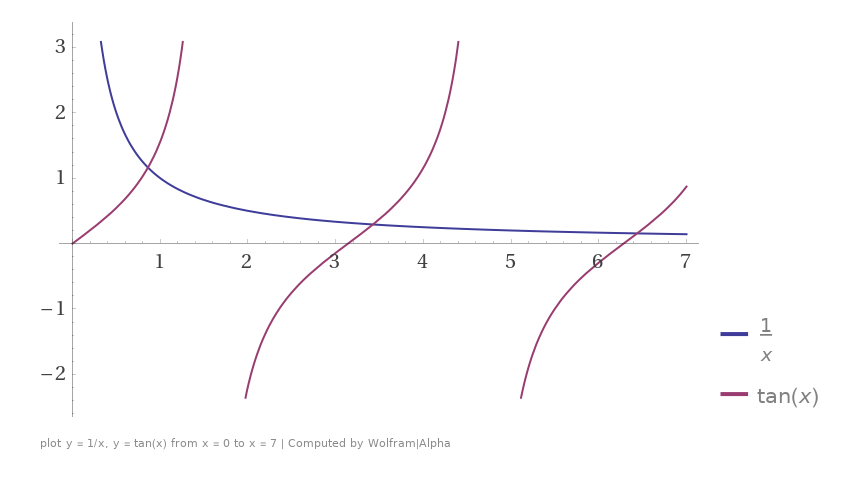
\includegraphics[width = 0.9 \textwidth]{4.png}
\end{center}

We therefore find that $\sqrt{\lambda_1} \approx 0.86$, $\sqrt{\lambda_2} \approx 3.43$ ... $\lambda_n \to \infty$

Therefore:

$$y(x) = \cos (\sqrt{\lambda} x) + \frac{h}{\sqrt{\lambda}} \sin( \sqrt{\lambda} x)$$

Hence we have $y_1 (x) \approx \cos (0.86x) + \frac{1}{0.86} \sin(0.86 x)$, etc. 

\section{Sturm - Liouville Problems involving the Cauchy - Euler equation}

\subsection{Example 17}

$$\mathcal{L} y = x^2 y'' + x y' + \lambda y = 0$$

Similar to what we have done in example 23, we can convert this to Sturm - Liouville format, such that it becomes $- (xy')' = \frac{\lambda}{x} y$

BCs: (1) $y(1) = 0$, (2) $y'(2) = 0$

Solution:

Guess a solution of $y = x^r$. Substitute this into the equation and we get the following:

$$\mathcal{L} x^r = x^r  \left(r(r-1) + r + \lambda \right) = 0$$

We need to therefore find roots of this equation:

$$\Rightarrow r^2 - r + r + \lambda = 0 \Rightarrow r^2 + \lambda = 0$$

If $\lambda > 0 \longrightarrow \lambda = \mu^2 \Rightarrow r = \pm i \mu$

This gets us a solution of $y(x) = x^{\pm i \mu} = e^{\pm - \mu \ln(x)}$ and therefore $y(x) = A \cos (\mu \ln x) + B\ sin(\mu \ln x)$. Substituting in the boundary conditions, from (1) we find that $A = 0$. Before we substitute the second, we find that $y'(x) = - \frac{A \mu}{x} \sin(\mu \ln x) + \frac{B \mu}{x} \cos(\mu \ln x)$. hence, substituting in (2) we find that $\frac{B \mu}{2} \cos(\mu \ln 2) = 0$ and therefore $\mu_n = \frac{(2n-1) \pi}{2 \ln 2}$ for $n \in \NN$. This gives us a general solution of the following:

$$y_n(x) = \sin \left[ \frac{2n-1) \pi}{2 \ln(2)} \ln(x) \right]$$

%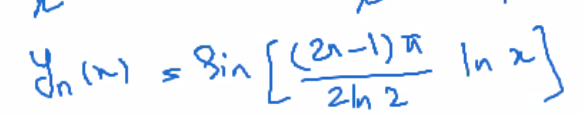
\includegraphics[width = 0.5 \textwidth]{2.png}

If $\lambda = 0$, $r^2 + \lambda = 0 \Rightarrow r = 0$ (repeated roots) and $y(x) = B + B \ln (x)$. From (1): $A = 0$ and from (2): $B = 0$ and hence we just get the trivial solution. 

\hfill

let's check the orthogonality of eigenfunctions:

$$r(x) = \frac{1}{x} \to \int_1^2 \frac{1}{x} \sin(\mu_k \ln (x)) \cdot \sin (\mu_m \ln(x)) dx = \left\{ \begin{matrix} 0 & k \neq m \\ \frac{\ln(2)}{2} & k = m \end{matrix} \right. = \frac{\ln(2)}{2} \delta_{km}$$

Note that $\delta$ is the Kronecker delta function. 

Proof regarding the previous integral: We use a change of variable $\ln x = u$. Then, $\frac{dx}{x} = du$. This integral therefore becomes:

$$\int_0^{\ln(2)} \sin(\mu_k u) \sin(\mu_m u) du = \frac{\ln(2)}{2} \delta_{km}$$

HINT: $\mu_n = \frac{(2n-1) \pi}{2 \ln(2)}$ and $\sin^2 (\alpha) = \frac{1}{2} \left[ 1 - \cos (2 \alpha) \right]$

\subsection{Example 28}

Solve the following Laplace's equation using boundary value problem in example 27. 

\begin{center}
    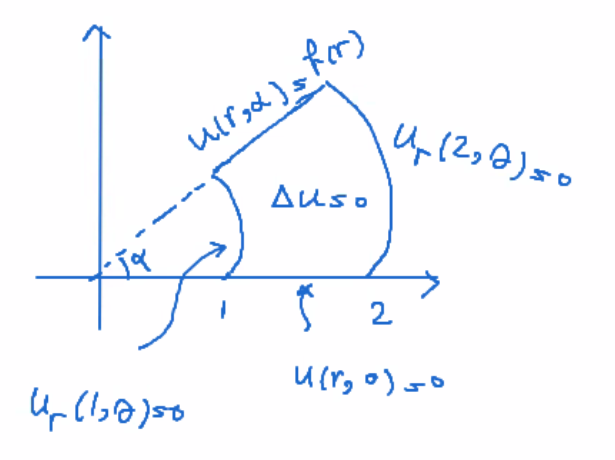
\includegraphics[width = 0.7 \textwidth]{3.png}
\end{center}

Using separation of variables:

$$- \left( \frac{r^2 R''}{R} + \frac{r R'}{R} \right) = \frac{\Theta''}{\Theta} = \lambda$$

R - function: $r^2 R'' + r R' + \lambda R = 0$. This is example 27. 

$R(1) = 0 = R'(2)$. From example 27, we know the solution is $\lambda = \mu^2 > 0$ and $\mu_n = \frac{(2n-1) \pi}{2 \ln (2)}$ and hence $R_n(r) = \sin \left( \mu_n \ln(r) \right)$

$\Theta$ - function: $\Theta'' - \lambda \Theta = 0 \Rightarrow \Theta(\theta) = A \cosh (\mu \theta) + B \sinh (\mu \theta)$. $A = 0$ and hence $\Theta_n (\theta) = B \sinh (\mu_n \theta)$

Superimposing the eigenfunctions:

$$u(r, \theta) = \sum_{n=1}^\infty B_n \sinh (\mu_n \theta) \sin(\mu_n \ln r)$$

BCs:

$$u(r, \alpha) = f(r) = \sum_{n=1}^\infty \underbrace{B_n \sinh (\mu_n \alpha)}_{b_n} \sin (\mu_n \ln(r))$$

Weight function: $r(x) = \frac{1}{r}$

$$b_n = \frac{\int_1^2 \frac{1}{r} f(r) \sin (\mu_n \ln r) dr}{\int_1^2 \frac{1}{r} \sin^2 (\mu_n \ln r) dr}$$

For this we use change of variable: $u = \ln r, du = \frac{dr}{r}$. 

$$\int_1^2 \frac{1}{r} \sin^2 (\mu_n \ln r) dr = \int_0^{\ln(2)} \sin^2 (\mu_n u) du = \frac{1}{2} \left[ u - \frac{1}{2 \mu_n} \sin \left( 2 \mu u \right) \right]_0^{\ln(2)} = \frac{\ln(2)}{2}$$

hence:

$$b_n = \frac{2}{\ln(2)} \int_1^2 \frac{1}{r} f(r) \sin (\mu_n \ln r) dr = b_n^{f(S-L)}$$

$$B_n = \frac{b_n^{f(S-L)}}{\sinh(\mu_n \alpha)}$$

Finally, we get the following:

$$u(r, \theta) = \sum_{n=1}^\infty \frac{b_n^{f(S-L)}}{\sinh(\mu_n \alpha)} \sinh (\mu_n \theta) \sin(\mu_n \ln r)$$

where $\mu_n = \frac{(2n-1) \pi}{2 \ln(2)}$ for $n \in \NN$

Exercise: $f(r) = 1$







\end{document}